%%%%%%%%%%%%%%%%%%%%%%%%%%%%%%%%%%%%%%%%%
% Thin Sectioned Essay
% LaTeX Template
% Version 1.0 (3/8/13)
%
% This template has been downloaded from:
% http://www.LaTeXTemplates.com
%
% Original Author:
% Nicolas Diaz (nsdiaz@uc.cl) with extensive modifications by:
% Vel (vel@latextemplates.com)
%
% License:
% CC BY-NC-SA 3.0 (http://creativecommons.org/licenses/by-nc-sa/3.0/)
%
%%%%%%%%%%%%%%%%%%%%%%%%%%%%%%%%%%%%%%%%%

%----------------------------------------------------------------------------------------
%	PACKAGES AND OTHER DOCUMENT CONFIGURATIONS
%----------------------------------------------------------------------------------------
\documentclass[12pt]{article} % Font size (can be 10pt, 11pt or 12pt) and paper size (remove a4paper for US letter paper)
\usepackage[protrusion=true,expansion=true]{microtype} % Better typography
\usepackage[left=1.1in,right=1.1in,top=1.1in,bottom=1.1in]{geometry}
\usepackage{graphicx} % Required for including pictures
\usepackage{wrapfig} % Allows in-line images
%\usepackage{mathpazo} % Use the Palatino font
\usepackage[T1]{fontenc} % Required for accented characters
%\linespread{1.05} % Change line spacing here, Palatino benefits from a slight increase by default
%\usepackage{array}
%\usepackage{booktabs}
%\usepackage{latexsym}
\usepackage{fancyhdr}
\usepackage{lastpage}
\usepackage[pdftex]{hyperref}
\usepackage{tipa}
\usepackage{url}
\usepackage{verbatim}
\hypersetup{
  colorlinks = true,
  urlcolor = black,
  citecolor=black,%
  filecolor=black,%
  linkcolor=black,%
  urlcolor=black     % can put red here to visualize the links
}
%\usepackage{biblatex}

\usepackage{outlines}
\usepackage{enumitem}

\newcounter{cenum}
\newcounter{cenumsaved}
\setcounter{cenumsaved}{0}
\newcommand{\labelcenum}{\arabic{cenum}.}
\newenvironment{cenumerate}%
{\begin{list}{\labelcenum}{\usecounter{cenum}}%
\setcounter{cenum}{\value{cenumsaved}}}%
{\setcounter{cenumsaved}{\value{cenum}}%
\end{list}}

\renewcommand{\outlineii}{cenumerate}

%\setenumerate[1]{label=\Roman*.}
%\setenumerate[2]{label=\Alph*.}
%\setenumerate[3]{label=\roman*.}
%\setenumerate[4]{label=\alph*.}

\makeatletter
%\renewcommand\@biblabel[1]{\textbf{#1.}} % Change the square brackets for each bibliography item from '[1]' to '1.'
\renewcommand{\@listI}{\itemsep=0pt} % Reduce the space between items in the itemize and enumerate environments and the bibliography

\renewcommand{\maketitle}{ % Customize the title - do not edit title and author name here, see the TITLE block below
\begin{center} % Right align
{\noindent\@title} % Increase the font size of the title

\vspace{10pt} % Some vertical space between the title and author name

{\noindent\@author}\\\@date

\vspace{10pt} % Some vertical space between the author block and abstract
\end{center}
}


%----------------------------------------------------------------------------------------
%	TITLE
%----------------------------------------------------------------------------------------
%\title{\LARGE{\textbf{Software Engineering Best Practices\\in Biomedical Informatics}\\[.5em]
%}}
%
%\author{\large{Nicholas J. Matiasz}\vspace{.4em}}
%
%\date{\large{2013-10-31}} % Date
%----------------------------------------------------------------------------------------

%----------------------------------------------------------------------------------------
%	HEADER/FOOTER
%----------------------------------------------------------------------------------------
\lhead{}
\chead{}
\rhead{}
\lfoot{BE 224A \textpipe\ Paper Review \#{1}}
\cfoot{\thepage\ of\ \pageref{LastPage}}
\rfoot{Nicholas J. Matiasz}
\renewcommand{\headrulewidth}{0.4pt}
\renewcommand{\footrulewidth}{0.4pt}
\pagestyle{fancyplain}

%----------------------------------------------------------------------------------------
%	ESSAY BODY
%----------------------------------------------------------------------------------------
\begin{document}

\begin{titlepage}

\newcommand{\HRule}{\rule{\linewidth}{0.5mm}} % Defines a new command for the horizontal lines, change thickness here

\center % Center everything on the page
 
%----------------------------------------------------------------------------------------
%	HEADING SECTIONS
%----------------------------------------------------------------------------------------

\textsc{\Large University of California, Los Angeles}\\[1.5cm] % Name of your university/college
\textsc{\large Medical Imaging Informatics Group}\\[0.5cm] % Major heading such as course name
\textsc{\large BE 224A Paper Review \#{1}}\\[0.5cm] % Minor heading such as course title

%----------------------------------------------------------------------------------------
%	TITLE SECTION
%----------------------------------------------------------------------------------------
\vspace{20pt}
\HRule \\[0.5cm]
\LARGE{\textbf{Paper Review:}}\\[.3cm]
\LARGE{\textbf{The Medawar Lecture, 2001}}\\[.3cm]
\LARGE{\textbf{by Richard L.\ Gregory}}\\
\HRule \\[1.5cm]
 
%----------------------------------------------------------------------------------------
%	AUTHOR SECTION
%----------------------------------------------------------------------------------------

\begin{minipage}{0.4\textwidth}
\begin{flushleft} \large
\emph{Author:}\\
Nicholas J.\ Matiasz % Your name
\end{flushleft}
\end{minipage}
~
\begin{minipage}{0.4\textwidth}
\begin{flushright} \large
\emph{Instructor:} \\
Prof.\ Ricky Taira % Supervisor's Name
\end{flushright}
\end{minipage}\\[4cm]

% If you don't want a supervisor, uncomment the two lines below and remove the section above
%\Large \emph{Author:}\\
%John \textsc{Smith}\\[3cm] % Your name

%----------------------------------------------------------------------------------------
%	DATE SECTION
%----------------------------------------------------------------------------------------
\begin{minipage}{0.4\textwidth}
\begin{center} \large
\emph{Submitted:} \\
2014-01-21 % Supervisor's Name
\end{center}
\end{minipage}\\[4cm]
%{\large Submitted: 2013-10-30}\\[3cm] % Date, change the \today to a set date if you want to be precise

%----------------------------------------------------------------------------------------
%	LOGO SECTION
%----------------------------------------------------------------------------------------
%\includegraphics{Logo}\\[1cm] % Include a department/university logo - this will require the graphicx package
%----------------------------------------------------------------------------------------
\vfill % Fill the rest of the page with whitespace
\end{titlepage}


\fontsize{12}{16}%22.5, 28
\selectfont
%\thispagestyle{empty}
%\tableofcontents

\section*{Summary of the 2001 Medawar Lecture}
The primary thesis of the 2001 Medawar Lecture \cite{gregory2005}, by Richard L.\ Gregory, is that the processes of image \textit{perception} and image \textit{interpretation} are rarely, if ever, fully decoupled, because our knowledge of the world significantly affects the way in which our visual systems operate. In other words, what we know---or at least believe to know---constrains what we see, and Gregory therefore laments that perception and learning are often studied as separate phenomena. This paper is divided into two complementary sections: the first addresses the concept of \textit{knowledge for vision}, and the second addresses \textit{vision for knowledge}. 

The first section describes various ways in which both our physiology and knowledge affect our perception.
Stating, ``we do not know by introspection what knowledge we use for perception,'' Gregory draws a distinction between conscious (explicit) understanding and unconscious (implicit) knowledge, and further highlights the entanglement of our eyes and brains.
He later presents the dichotomy of explicit and implicit knowledge with the categories of \textit{conceptual} and \textit{visual}, respectively.

Examples of unconscious or implicit knowledge are often illuminated via illusions, which occur when our perception comes into conflict with facts that we hold about the world. Gregory presents many examples of these illusions in turn, including those derived from bottom-up signals (e.g., jazzing, retinal rivalry, and local drifting), and those derived from top-down knowledge (e.g., familiarity blindness, constancy, and pseudo-parallax). Gregory is careful to differentiate illusions from \textit{optical} illusions, which he defines specifically as ``disturbances of light between the object and the eyes.'' It is by studying illusions, or ``perceptual departures from physics,'' that we can understand with greater subtlety the inner workings of our perceptual systems because they help us to distinguish physical phenomena from perceptual phenomena. Confusion remains as to whether some of these illusions result from errors that are either physiological (bottom-up) or cognitive (top-down) in nature.  

An aspect of the human visual system that gives researchers access to its design is the concept of stability---also called constancy. Our visual system achieves this stability by compensating for certain changes in the visual field, often to normalize perception. However, these visual compensations are not always appropriate given the physical context of the perceived phenomena. When the brain enforces these corrections at inappropriate times, the result is often a perceptual error that is in some way the opposite of the phenomena that is usually corrected. An example of this process is the \textit{Ouchi illusion}, in which the orthogonality and differing spatial frequency of channels in the visual field can give the illusion of motion. An example of this illusion can be seen in Figure \ref{ouchi}.

\begin{figure}[h]
\centering
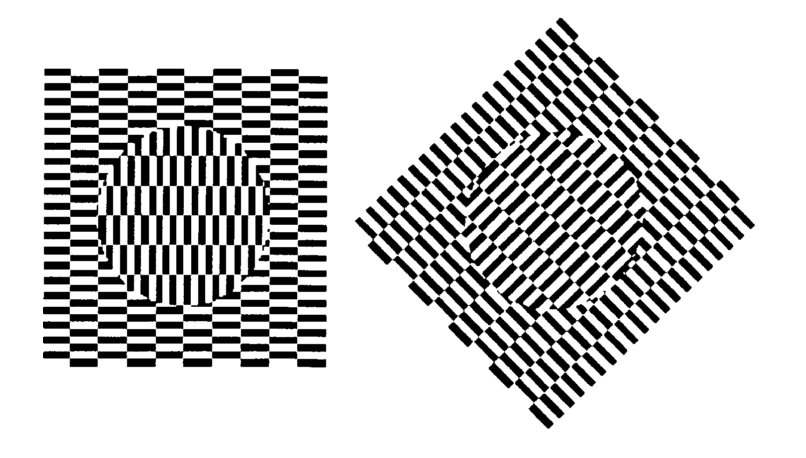
\includegraphics[scale=.40]{./images/ouchi.png}
\caption{Ouchi illusion}
\label{ouchi}
\end{figure}

In the second part of this text, Gregory discusses the complementary idea of using vision as a means for gaining knowledge about the world. 
Despite vision's obvious utility for a variety of human pursuits, Gregory points out an interesting fact: ``Inputs [i.e., visual appearances] can inhibit imagination.'' This idea highlights an subtle tension that pervades our daily experience---namely, that we need prior knowledge for our vision to be meaningful, and yet we so often rely on our vision to further our knowledge about the world. In addition to the dichotomy of conscious-vs.-unconscious knowledge, Gregory describes visual knowledge with two categories: \textit{specific} knowledge, which always refers to a certain object in the world, and \textit{rules} (e.g., \textit{perspective}), which describe sets of objects and can be applied in a variety of circumstances. The rules that an individual forms throughout life therefore depend on the dynamics of this vision-knowledge interplay.

\pagebreak[4]

\section*{Outline of the 2001 Medawar Lecture}
\begin{minipage}[t]{0.45\linewidth}
\begin{outline}
   \1 Part I
      \2 Knowledge for vision
         \3 Outline evolution
         \3 Ancient and modern streams of brain processing
         \3 Seeing pictures
         \3 Knowledge
         \3 `Physiological' and `cognitive'
         \3 Ins-and-outs of vision
         \3 Illusions
         \3 Classifying illusions
      \2 Non-sense
      	\3 Total (bottom-up) blindness
      	\3 Agnosia (top-down blindness)
      	\3 Neglect
      	\3 Blindsight
      \2 Instability
      	\3 Border locking?
      	\3 After-effects
      	\3 Jazzing
      	\3 Eye movements
      	\3 Auto-kinetic effect
      	\3 Self-movement and object-movement
      	\3 Motion parallax
      	\3 Stereoscopic vision
      	\3 Pseduo-parallax
      	\3 Portrait eyes
      	\3 Reverspectives
\end{outline}
\end{minipage}
\hspace{0.5cm}
\begin{minipage}[t]{0.45\linewidth}
\begin{outline}
	\1 Part I (continued)
	\2 Contrast
	\2 Confounded ambiguity
      	\3 The Ames Room
      \2 Flipping ambiguity
      	\3 Wire cube
      	\3 Hollow face
     	\2 Distortion
     		\3 Physiological distortions
     		\3 Cognitive distortions
      \2 Grouping
      \2 Glass effect
      \2 Impossible
      \2 Fiction
      	\3 Filling-in
      	\3 Phantasms
      	\3 Peeriodic table
     \setcounter{cenum}{0}
 	\1 Part II
 		\2 Vision for knowledge
\end{outline}
\end{minipage}



%----------------------------------------------------------------------------------------
%	BIBLIOGRAPHY
%----------------------------------------------------------------------------------------
\bibliographystyle{plain}
\bibliography{224a_paper_review_1}
%----------------------------------------------------------------------------------------

\end{document}